\subsection{Mujoco}

Mujoco is released in 2015, making it the newest physics engine in our comparison. It stands for Multi-Joint Control. Hence the name, its primary purpose, is Robot simulation.
 
We first considered Mujoco as our main simulator. Our consideration was based on; Roboticist mainly using Mujoco at OpenAI and DeepMind \cite{OpenAIgym}. Besides, simulation engine reviews featured Mujoco as the best performing and stable engine \cite{Erez2015}. Erez et al. conducted tests that compared the performance of physics engines on grasping tasks, where Mujoco by far performed better than the other engines \ref{fig:handmujoco}. Additionally, Mujoco provides an API that lets users develop in C language. C language API is a significant advantage for researchers aim to get as close to the hardware as possible to save time. Another plus is mujoco-py offers a Python API to control Mujoco simulation easily. OpenAI product Mujoco-py\footnote{\url{https://github.com/openai/mujoco-py}} is entirely open-source with MIT license. 

\begin{figure}[htbp]
    \centering
      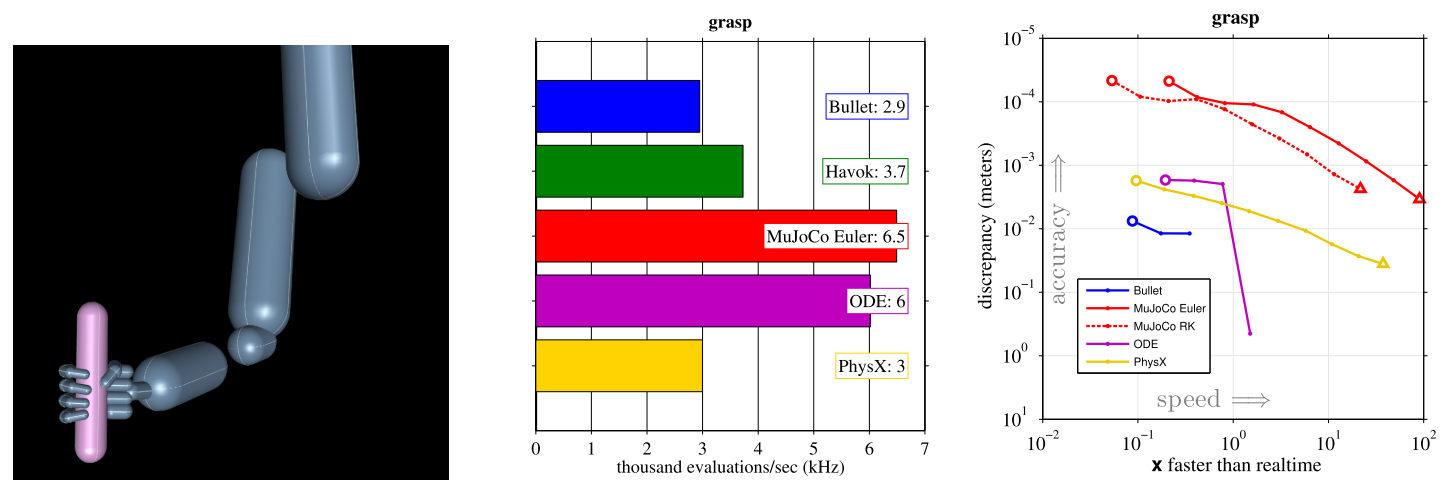
\includegraphics[width=1.0\textwidth]{figures/MujocoHand}
    \caption{physics engine performance on grasping task. Mujoco performs the best \cite{Erez2015}}
    \label{fig:handmujoco}
\end{figure}


On the other hand, MuJoCo requires a license to use for research purposes. Personal non-commercial license costs \(500\$\) as of 2020 July. License cost is the main drawback because we prefer complete open-source software. Another factor is the training time since our models require over 10M time-steps to train, we need to make use of every millisecond time gain in every step. So, GPU support is highly crucial. Mujoco only supports CPU simulation, which has the potential to be slower than GPU. As a side-note, we have not compared the MuJoCo CPU version speed with Bullet GPU version speed. MuJoCo developers prepared a performance page where they explain the GPU vs. CPU comparison. They pointed out that if decoupled systems are simulated like particle simulation, GPU has an advantage. Whereas, one simulates coupled system such as a humanoid robot CPU gain a slight edge \ref{fig:mujococpu}. They also noted that there is room for research in the areas besides coupled or decoupled systems\footnote{\url{http://mujoco.org/performance.html}}.

\begin{figure}[htbp]
    \centering
      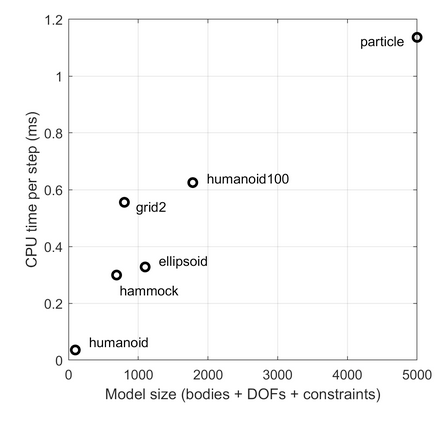
\includegraphics[width=0.7\textwidth]{figures/MujocoCPU1}
    \caption{CPU time per step comparison of different tasks \cite{Erez2015}}
    \label{fig:mujococpu}
\end{figure}

Finally, observing large open-source projects like OpenAI-Roboschool, which initially used MuJoCo, deprecating, and suggesting PyBullet, made us reconsider. We believe that the reason community migrating towards PyBullet is completely open-source codebase. 

\begin{figure}[htbp]
    \centering
      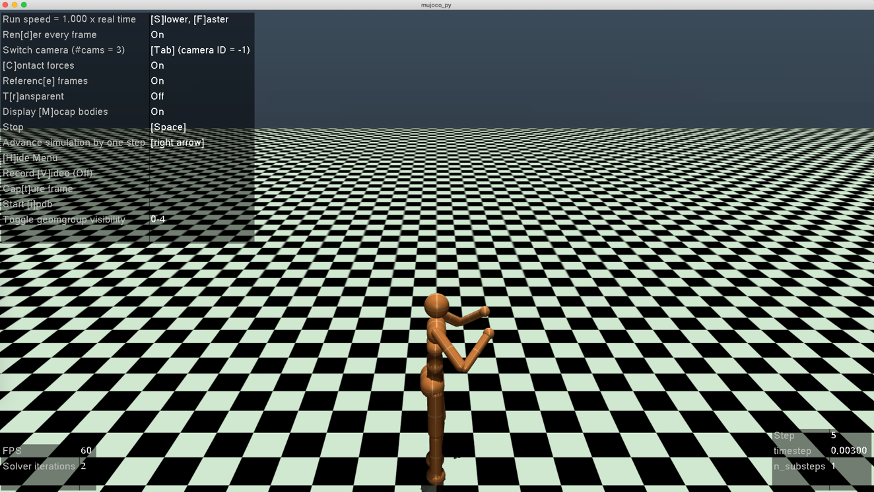
\includegraphics[width=1.\textwidth]{figures/MujocoHuman1}
    \caption{Mujoco simulation of a humanoid model. Rendered with MJViewer}
    \label{fig:mujocohuman}
\end{figure}